% !TeX root = ../Tempel-Daniel.tex
\chapter{Context Engineering and Memory}
\label{chap:context-memory}

The previous chapter showed how structured tool calls allow the AI Software Engineering Assistant to interact with repositories, APIs and test runners. Each interaction can add issue descriptions, search results, source files, patches and test output to subsequent model requests. The resulting architectural problem is therefore not only how the assistant obtains information, but which information should be available to the LLM for its next decision.

Chapter~\ref{chap:local-llms} introduced the context window as a runtime constraint and distinguished the model-supported maximum context length, the runtime-configured context size and the active context of an individual request. Context engineering addresses the selection, organisation and maintenance of the information that occupies this context. Anthropic distinguishes it from prompt engineering: while prompt engineering primarily concerns the formulation of instructions, context engineering also includes tool definitions, interaction history and external information \parencite{anthropic2025context}.

For a tool-using assistant, the goal is therefore to provide a relevant and sufficient set of information for the current decision within the available context budget.

\section{Constructing the active context}
\label{sec:active-context}

During a software-engineering task, more information may be available than should be included in a single request. Potential inputs include system and project instructions, the user request, tool definitions, previous interactions, repository files, source-code changes, tool results and retained information from earlier work. A context-building stage can select from these sources before invoking the LLM.

\noindent\begin{minipage}{\linewidth}
\centering
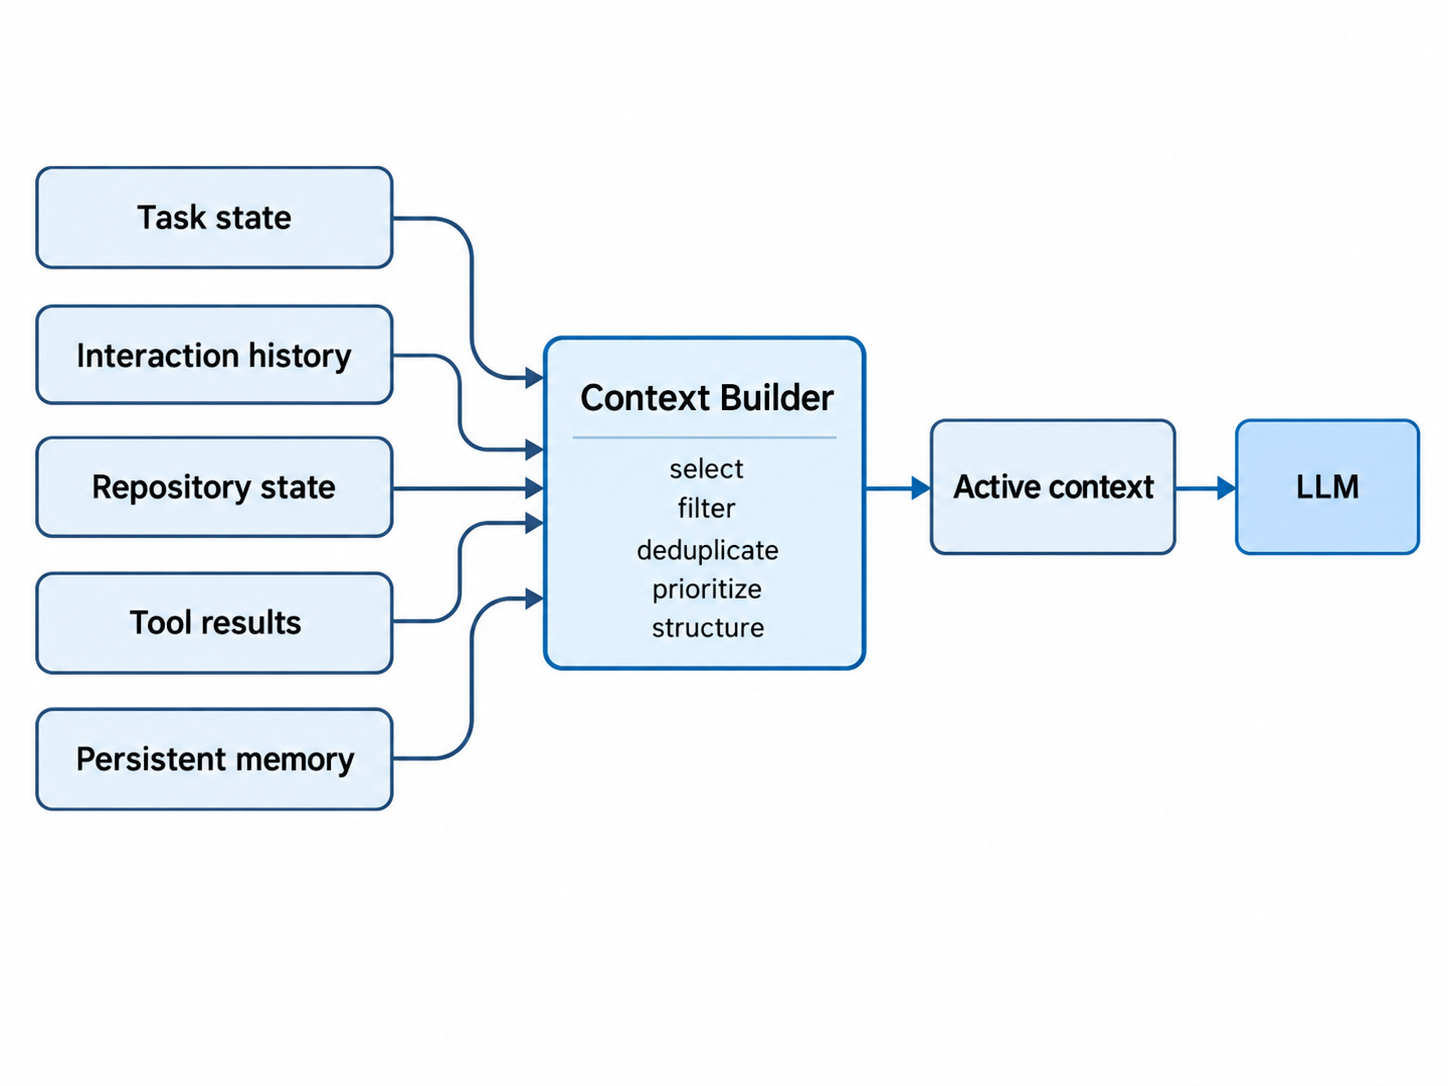
\includegraphics[width=\linewidth,trim=15bp 240bp 15bp 145bp,clip]{images/context-builder.png}
\captionsetup{hypcap=false}
\captionof{figure}{Construction of the active context from task state, interaction history, repository information, tool results and persistent memory.}
\label{fig:active-context-construction}
\end{minipage}

A context policy can distinguish information that should remain available throughout a task, such as the objective, explicit user constraints and relevant project rules, from information selected dynamically for the current step. Excluded detail should remain recoverable from its original source if it later becomes relevant.

Consider the recurring task \emph{Fix GitHub issue \#42 and verify the solution}. Initially, the active context may contain the issue description, project instructions and tools such as \texttt{search\_code}, \texttt{read\_file}, \texttt{apply\_patch} and \texttt{run\_tests}. If the issue concerns incorrect handling of an \texttt{Authorization} header, a code search may identify \texttt{src/auth.py} and related tests. After these files have been inspected, the complete search output may be replaced by the relevant source code, observed behaviour and current hypothesis. After a patch, the current diff and verification state become more important than earlier exploratory results.

Context construction is therefore iterative. Each tool interaction changes the available state and may change which information is useful for the next inference step. Tool interfaces should support this by filtering, paginating or limiting low-value output, while excessively broad or overlapping tool sets can also consume context and make tool selection more ambiguous \parencite{anthropic2025tools}.

A larger supported context window does not remove the need for selection. In the models and tasks evaluated by \textcite{liu2024lostmiddle}, the position of relevant information affected performance, with information in the middle of long contexts often being used less reliably. RULER likewise observed degradation with increasing sequence length and task complexity in the evaluated models \parencite{hsieh2024ruler}. Maximum context length should therefore be treated as a capacity limit rather than a target.

These choices also form part of the context policy introduced in Chapter~\ref{chap:benchmarks} and should remain controlled when candidate models are compared.

\section{History, task state and persistent memory}
\label{sec:history-memory}

Long-running tool interaction requires distinguishing different roles of retained information. Interaction history records what happened, task state represents information needed to continue the current task, and persistent memory refers here to selected information retained for reuse beyond the immediate task state. These are functional roles rather than mutually exclusive storage mechanisms; history and task state may themselves also be persisted.

The complete interaction history can contain messages, tool calls, raw search results and repeated test runs. It may remain available to the assistant runtime for audit, debugging or later retrieval without being included in every model request. Stored history and active context are therefore separate architectural concerns.

Task state should preserve the information required to continue coherently, such as the current goal, user constraints, inspected files, applied changes and verification status. Some of this state consists of operational facts that the runtime can record directly. Other information, such as an assumed root cause, is a model-derived hypothesis. Storing a hypothesis in a structured checkpoint does not make it an observed fact.

Structured checkpoints should therefore preserve the status of the information they contain. They can record, for example, that \texttt{src/auth.py} was modified and a test was executed while keeping the suspected relationship between the change and issue \#42 explicitly marked as a hypothesis until verified.

Verification state is also tied to the code state that was tested. If relevant code is modified afterwards, an earlier passing test remains a valid historical observation but no longer verifies the current version and may need to be repeated.

Persistent memory retains selected information useful for future work, such as repository conventions or recurring project-specific procedures. In a Java project, the command used to run tests may be reusable knowledge, while an intermediate test failure is usually temporary task state. MemGPT illustrates the broader principle of treating the model context as a limited working tier while moving information between it and larger external storage \parencite{packer2023memgpt}.

Persistent memory therefore requires policies for retention, retrieval, update and invalidation. Provenance is important: if stored memory states that a project uses Java 17 while the current \texttt{pom.xml} specifies Java 21, the current repository state is the more authoritative source.

Treating every stored observation as reusable memory would create an increasingly noisy retrieval source, even if the complete interaction history remains useful as an archive. Persistent memory should therefore favour information that is stable, reusable and worth retaining.

\section{Compaction and context efficiency}
\label{sec:compaction-efficiency}

Even with selective context construction, long tool interactions can produce more useful history than should remain verbatim in every request. Compaction addresses this by replacing part of the previous context with a smaller representation that preserves the information required to continue the task.

For a software-engineering assistant, compacted state should retain the goal, explicit user constraints, scope boundaries, acceptance criteria, important findings, relevant source references, architectural decisions, modified files, verification results and unresolved problems. It should also preserve distinctions between observed facts, hypotheses and unverified interpretations. Obsolete search results, duplicated source snippets, superseded hypotheses and large intermediate logs can often be removed.

Anthropic describes compaction as preserving important decisions and unresolved work while discarding redundant information, including old tool results \parencite{anthropic2025context}. OpenAI likewise provides compaction for long-running interactions to reduce context while carrying forward state required by later turns \parencite{openai-compaction}.

Compaction is inherently lossy. A smaller representation reduces token usage and irrelevant information, but may discard details that later become useful. Structured checkpoints can reduce this risk for explicitly recorded operational facts, while the original interaction history can remain stored outside the active context for later recovery.

\noindent\begin{minipage}{\linewidth}
\centering
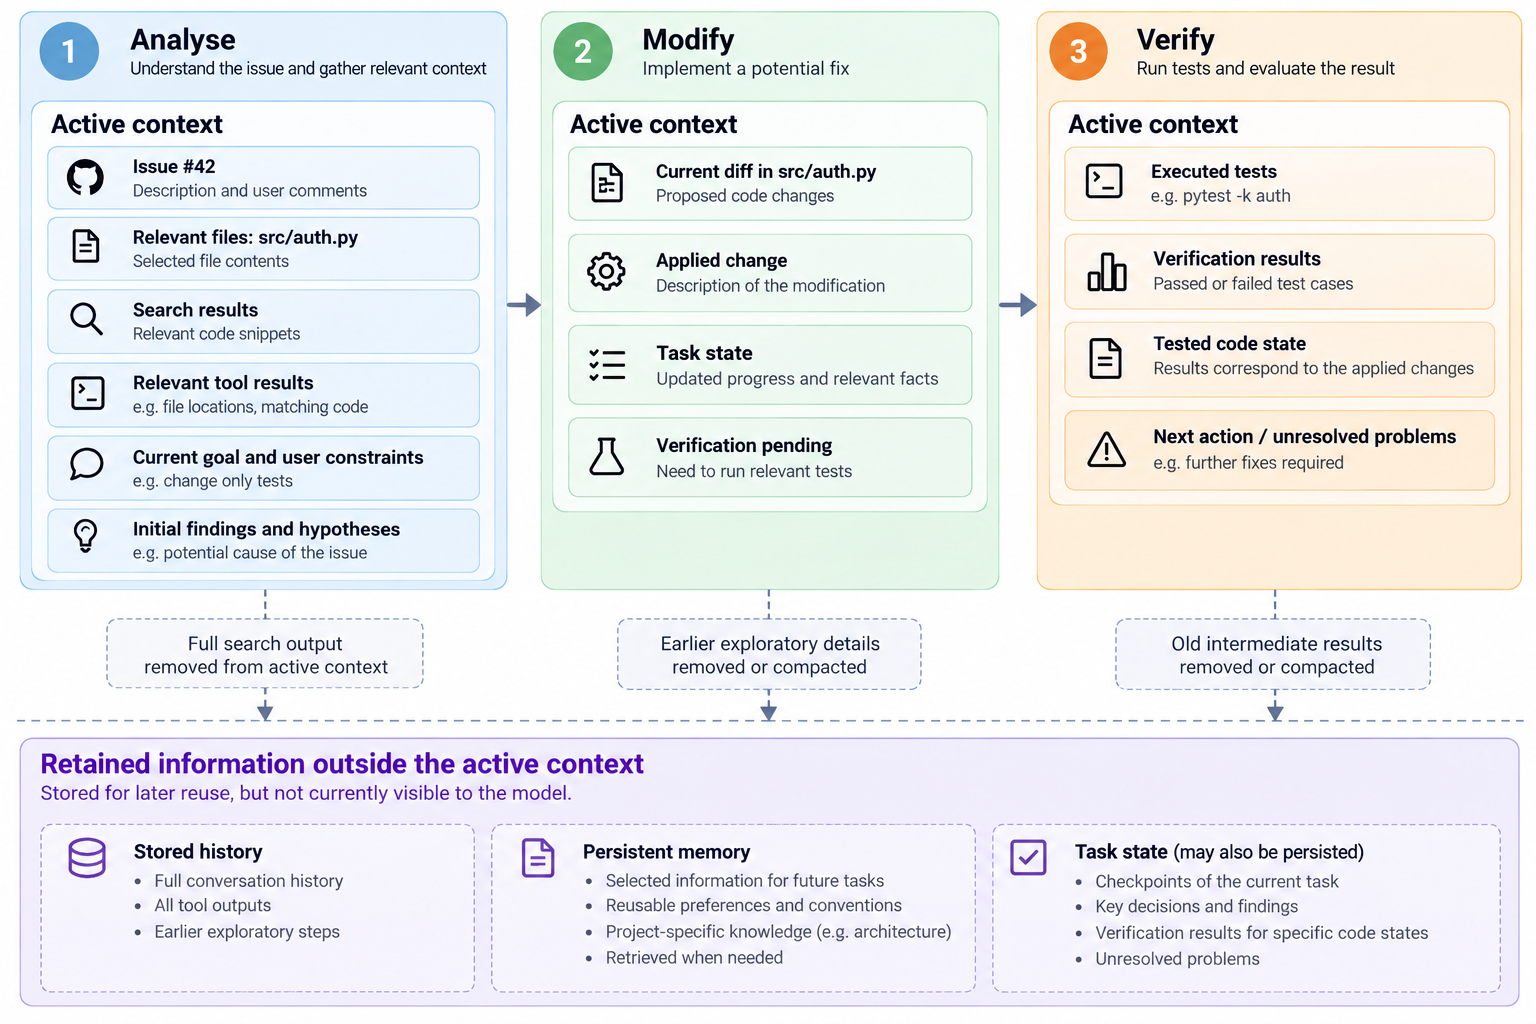
\includegraphics[width=\linewidth]{images/context-evolution.png}
\captionsetup{hypcap=false}
\captionof{figure}{Evolution of the active context while analysing, modifying and verifying GitHub issue \#42.}
\label{fig:active-context-evolution}
\end{minipage}

Prompt caching addresses a separate efficiency problem. The KV cache introduced in Chapter~\ref{chap:local-llms} stores attention key-value states during inference. Prompt caching can reuse previously computed states across model requests that share a cacheable prefix, although the exact mechanism depends on the runtime or API provider. Stable information such as system instructions, project rules and tool definitions can therefore benefit from repeated prefix reuse \parencite{openai-prompt-caching}.

Prompt caching does not increase context capacity. Cached input still occupies the model's context window; caching reduces repeated computation rather than the amount of information presented to the model. Persistent memory, compaction and prompt caching therefore solve different problems.

These mechanisms can also interact. Compaction may reduce input tokens but alter part of the previously reusable prefix, while an unchanged earlier prefix may remain cacheable. Context management is therefore an optimisation across model quality, context usage, latency and computational reuse rather than a simple attempt to minimise token count.

These considerations suggest an architecture in which the AI Software Engineering Assistant should maintain explicit task state, select information relevant to the current step, retrieve reusable persistent information when required and compact interaction history as a task grows. The remaining question is how the assistant can efficiently locate external information not already present in its active context. This leads to retrieval-augmented generation and agentic retrieval, examined in the following chapter.
